% Generated by make_results_figures.py from media/data/*.json.
% Those numbers are DIGITIZED from the published figures, not the
% original data: see media/data/README.md.
\documentclass[border=6pt]{standalone}
\usepackage[T1]{fontenc}
\usepackage{helvet}
\renewcommand{\familydefault}{\sfdefault}
\usepackage{amsmath}
\usepackage{tikz}
\usetikzlibrary{arrows.meta,calc,decorations.pathreplacing}
\definecolor{spaceC}{HTML}{3B6EA5}
\definecolor{timeC}{HTML}{D9822B}
\definecolor{hcC}{HTML}{6B5B95}
\definecolor{vcC}{HTML}{8A7F72}
\definecolor{ink}{HTML}{2B2B2B}
\definecolor{muted}{HTML}{6B6B6B}
\definecolor{gridC}{HTML}{E6E4E0}
\definecolor{nanC}{HTML}{EFEDEA}
\definecolor{s1}{HTML}{2A78D6}
\definecolor{s2}{HTML}{EB6834}
\definecolor{s3}{HTML}{1BAF7A}
\definecolor{s4}{HTML}{EDA100}
\definecolor{s5}{HTML}{E87BA4}
\begin{document}
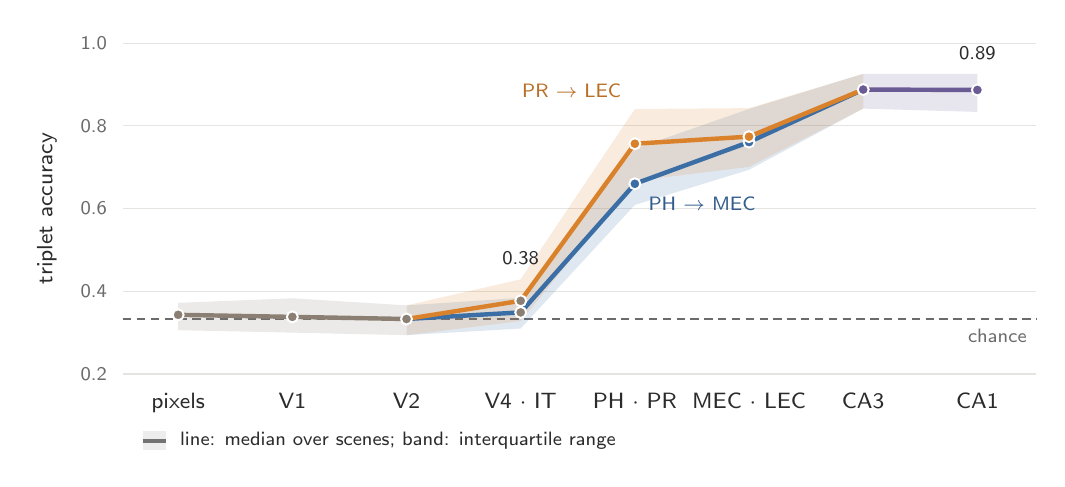
\begin{tikzpicture}[font=\footnotesize,
  tick/.style={font=\scriptsize,text=muted},
  lab/.style={font=\footnotesize,text=ink},
  ttl/.style={font=\small\bfseries,anchor=west,text=ink}]

\draw[gridC,line width=0.4pt] (0.000,0.000)--(11.600,0.000);
\node[tick,anchor=east] at (-0.080,0.000) {0.2};
\draw[gridC,line width=0.4pt] (0.000,1.050)--(11.600,1.050);
\node[tick,anchor=east] at (-0.080,1.050) {0.4};
\draw[gridC,line width=0.4pt] (0.000,2.100)--(11.600,2.100);
\node[tick,anchor=east] at (-0.080,2.100) {0.6};
\draw[gridC,line width=0.4pt] (0.000,3.150)--(11.600,3.150);
\node[tick,anchor=east] at (-0.080,3.150) {0.8};
\draw[gridC,line width=0.4pt] (0.000,4.200)--(11.600,4.200);
\node[tick,anchor=east] at (-0.080,4.200) {1.0};
\node[lab,rotate=90,anchor=south] at (-0.720,2.100) {triplet accuracy};
\draw[muted,densely dashed,line width=0.5pt] (0,0.700)--(11.600,0.700);
\node[tick,anchor=north east] at (11.600,0.700) {chance};
\fill[vcC,opacity=0.16] (0.700,0.903) -- (2.150,0.961) -- (3.600,0.871) -- (3.600,0.493) -- (2.150,0.525) -- (0.700,0.556) -- cycle;
\fill[spaceC,opacity=0.16] (3.600,0.871) -- (5.050,0.966) -- (6.500,2.861) -- (7.950,3.365) -- (9.400,3.812) -- (9.400,3.370) -- (7.950,2.593) -- (6.500,2.147) -- (5.050,0.577) -- (3.600,0.493) -- cycle;
\fill[timeC,opacity=0.16] (3.600,0.871) -- (5.050,1.202) -- (6.500,3.365) -- (7.950,3.376) -- (9.400,3.812) -- (9.400,3.370) -- (7.950,2.630) -- (6.500,2.452) -- (5.050,0.672) -- (3.600,0.493) -- cycle;
\fill[hcC,opacity=0.16] (9.400,3.812) -- (10.850,3.812) -- (10.850,3.328) -- (9.400,3.370) -- cycle;
\draw[vcC,line width=1.6pt,line join=round,line cap=round] (0.700,0.751) -- (2.150,0.725) -- (3.600,0.698);
\draw[spaceC,line width=1.6pt,line join=round,line cap=round] (3.600,0.698) -- (5.050,0.782) -- (6.500,2.415) -- (7.950,2.945) -- (9.400,3.612);
\draw[timeC,line width=1.6pt,line join=round,line cap=round] (3.600,0.698) -- (5.050,0.929) -- (6.500,2.924) -- (7.950,3.014) -- (9.400,3.612);
\draw[hcC,line width=1.6pt,line join=round,line cap=round] (9.400,3.612) -- (10.850,3.607);
\filldraw[fill=vcC,draw=white,line width=0.7pt] (0.700,0.751) circle (0.07);
\filldraw[fill=vcC,draw=white,line width=0.7pt] (2.150,0.725) circle (0.07);
\filldraw[fill=vcC,draw=white,line width=0.7pt] (3.600,0.698) circle (0.07);
\filldraw[fill=vcC,draw=white,line width=0.7pt] (5.050,0.782) circle (0.07);
\filldraw[fill=vcC,draw=white,line width=0.7pt] (5.050,0.929) circle (0.07);
\filldraw[fill=spaceC,draw=white,line width=0.7pt] (6.500,2.415) circle (0.07);
\filldraw[fill=timeC,draw=white,line width=0.7pt] (6.500,2.924) circle (0.07);
\filldraw[fill=spaceC,draw=white,line width=0.7pt] (7.950,2.945) circle (0.07);
\filldraw[fill=timeC,draw=white,line width=0.7pt] (7.950,3.014) circle (0.07);
\filldraw[fill=hcC,draw=white,line width=0.7pt] (9.400,3.612) circle (0.07);
\filldraw[fill=hcC,draw=white,line width=0.7pt] (10.850,3.607) circle (0.07);
\node[tick,text=spaceC!85!black,anchor=north west] at (6.550,2.365) {PH $\to$ MEC};
\node[tick,text=timeC!85!black,anchor=south east] at (6.450,3.385) {PR $\to$ LEC};
\node[tick,text=ink,anchor=south] at (10.850,3.872) {0.89};
\node[tick,text=ink,anchor=south] at (5.050,1.262) {0.38};
\node[lab,anchor=north] at (0.700,-0.12) {pixels};
\node[lab,anchor=north] at (2.150,-0.12) {V1};
\node[lab,anchor=north] at (3.600,-0.12) {V2};
\node[lab,anchor=north] at (5.050,-0.12) {V4 $\cdot$ IT};
\node[lab,anchor=north] at (6.500,-0.12) {PH $\cdot$ PR};
\node[lab,anchor=north] at (7.950,-0.12) {MEC $\cdot$ LEC};
\node[lab,anchor=north] at (9.400,-0.12) {CA3};
\node[lab,anchor=north] at (10.850,-0.12) {CA1};
\fill[black!45,opacity=0.16] (0.250,-0.97) rectangle (0.550,-0.73);
\draw[black!55,line width=1.6pt] (0.250,-0.85)--(0.550,-0.85);
\node[tick,text=ink,anchor=west] at (0.600,-0.85) {line: median over scenes; band: interquartile range};
\end{tikzpicture}
\end{document}

